\documentclass[tikz,border=3pt]{standalone}
\usepackage[T1]{fontenc}
\usepackage{amsmath}
\usepackage{XCharter}
\usepackage[xcharter]{newtxmath}
\usepackage[scaled=.92]{helvet}
\usepackage{pgfplots}
\usetikzlibrary{arrows.meta,positioning,fit,calc,backgrounds,decorations.pathreplacing,patterns}
\usepgfplotslibrary{groupplots,fillbetween}
\pgfplotsset{compat=1.18}
\definecolor{ink}{HTML}{172536}
\definecolor{rgb}{HTML}{3563B8}
\definecolor{event}{HTML}{17857C}
\definecolor{fusion}{HTML}{76529C}
\definecolor{reference}{HTML}{8994A3}
\definecolor{warn}{HTML}{AC5948}
\definecolor{muted}{HTML}{657183}
\definecolor{rule}{HTML}{D9E0E8}
\definecolor{pale}{HTML}{F5F7FA}
\color{ink}
\tikzset{box/.style={rounded corners=2pt,draw=rule,fill=white,align=center,inner sep=4pt,font=\sffamily\fontsize{9}{10.8}\selectfont,minimum height=9mm},rb/.style={box,draw=rgb!50,fill=rgb!5},eb/.style={box,draw=event!50,fill=event!5},fb/.style={box,draw=fusion!55,fill=fusion!5},arrow/.style={-{Latex[length=1.8mm]},line width=.65pt,draw=muted},note/.style={font=\sffamily\fontsize{8.4}{10.2}\selectfont,align=center,text=muted},heading/.style={font=\sffamily\fontsize{10}{12}\selectfont\bfseries,align=left,text=ink}}
\pgfplotsset{paper/.style={width=15.7cm,height=6cm,axis lines*=left,axis line style={rule},tick style={draw=none},tick label style={font=\sffamily\fontsize{8.8}{10.4}\selectfont,text=muted},label style={font=\sffamily\fontsize{9.4}{11}\selectfont,text=ink},title style={font=\sffamily\fontsize{10}{12}\selectfont\bfseries,text=ink},legend style={draw=none,fill=none,font=\sffamily\fontsize{9}{11}\selectfont,cells={anchor=west}},grid=major,grid style={rule!65,line width=.3pt},minor tick num=0,scaled ticks=false,unbounded coords=jump,clip mode=individual}}
\begin{document}

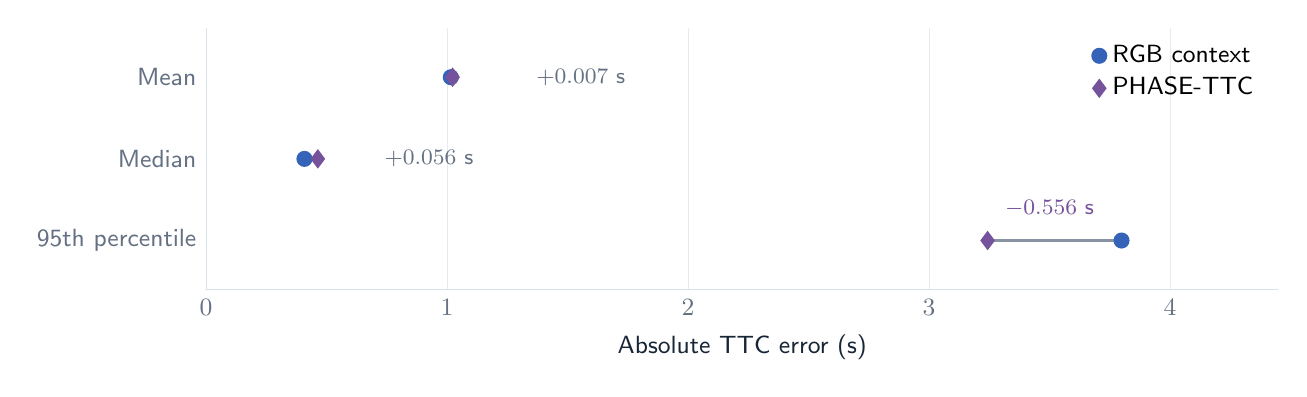
\begin{tikzpicture}
\begin{axis}[paper,width=15.2cm,height=4.9cm,xmin=0,xmax=4.45,ymin=-.6,ymax=2.6,ytick={0,1,2},yticklabels={95th percentile,Median,Mean},xlabel={Absolute TTC error (s)},xtick={0,1,2,3,4},ymajorgrids=false,legend style={at={(.99,.98)},anchor=north east}]
\addplot[reference,line width=1pt,forget plot] coordinates {(3.24301000583191,0) (3.79878091916809,0)};
\addplot[reference,line width=1pt,forget plot] coordinates {(0.463565129631043,1) (0.407897321632385,1)};
\addplot[reference,line width=1pt,forget plot] coordinates {(1.02267728914496,2) (1.01537748105316,2)};
\addplot[only marks,mark=*,mark size=2.7pt,rgb] coordinates {(3.79878091916809,0) (0.407897321632385,1) (1.01537748105316,2)};\addlegendentry{RGB context}
\addplot[only marks,mark=diamond*,mark size=3.2pt,fusion] coordinates {(3.24301000583191,0) (0.463565129631043,1) (1.02267728914496,2)};\addlegendentry{PHASE-TTC}
\node[note,text=fusion,anchor=south] at (axis cs:3.5,.17) {\(-0.556\) s};
\node[note,anchor=west] at (axis cs:.7,1) {\(+0.056\) s};
\node[note,anchor=west] at (axis cs:1.33,2) {\(+0.007\) s};
\end{axis}
\end{tikzpicture}
\end{document}
